% =====================================================================
%  FloodLite: A Multi-Platform Edge-Deployment Benchmark for
%             Lightweight Flood Segmentation
%  Author: Md Ibrahim Khalil (lead)
%  Target venue: Elsevier International Journal of Disaster Risk
%                Reduction (IJDRR), primary.
%  Backup venue: IGARSS 2026 (4-page extended abstract).
%  Numbers source of truth:
%       code/runs/3fold/{summary,quantized,lat_m2,lat_wasm}.json
%  Tables source of truth: docs/tables.md
%  Status: v2 draft (post edge-benchmark pivot, 2026-05-16).
% =====================================================================

% IJDRR camera-ready style: Elsevier two-column journal format
% (final, 3p = double-column, times font).  Use [preprint,review,12pt]
% during review-with-line-numbers; switch to [final,3p,times] for the
% submission-ready look that matches what published IJDRR papers look like.
\documentclass[final,3p,times,twocolumn]{elsarticle}

% ---------- Packages ----------
\usepackage[T1]{fontenc}
\usepackage[utf8]{inputenc}
\usepackage[british]{babel}
\usepackage{graphicx}
\usepackage{amsmath,amssymb}
\usepackage{booktabs}
\usepackage{array}
\usepackage{url}
\usepackage{xcolor}
\usepackage[hidelinks]{hyperref}
\usepackage{textcomp}
\usepackage{tabularx}
\usepackage{caption}
\usepackage{multirow}
\usepackage{siunitx}
\sisetup{detect-weight=true,detect-family=true}
\usepackage{microtype}            % subtle character protrusion + font expansion

% ---------- Macros for FloodLite numbers ----------
% Headline numbers; update here and they propagate through the text.
\newcommand{\teacherIoU}{0.9257}
\newcommand{\teacherStd}{0.0078}
\newcommand{\bestStudentIoU}{0.9367}
\newcommand{\bestStudentStd}{0.0055}
\newcommand{\bestStudent}{MobileViT-XXS}
\newcommand{\deployableModel}{EfficientNet-Lite0}
\newcommand{\deployableINTIoU}{0.8851}
\newcommand{\deployableINTStd}{0.0149}
\newcommand{\deployableINTDelta}{-0.0426}
\newcommand{\deployableMTwoFPS}{58}
\newcommand{\deployableWASMFPS}{6}
\newcommand{\teacherMTwoFPS}{26.6}  % teacher ORT-CPU FPS (ORT 1.17); PyTorch-eager was 3.6

% Convenience commands.
\newcommand{\Cn}{C\textsubscript{n}}
\newcommand{\ie}{i.e.,\ }
\newcommand{\eg}{e.g.,\ }

% ---------- Front matter ----------
\journal{International Journal of Disaster Risk Reduction}

\begin{document}

% Allow TeX to break lines more loosely; tight column justification
% with long \texttt{} paths otherwise produces huge inter-word gaps.
\sloppy

\begin{frontmatter}

\title{FloodLite: A Multi-Platform Edge-Deployment Benchmark for Lightweight Flood Segmentation}

\author[sensa]{Md Ibrahim Khalil\corref{cor1}}
\ead{ibrahim@sensa.no}

% Add co-authors here when finalised:
% \author[affB]{Co-Author Two}
% \author[affC]{Co-Author Three}

\affiliation[sensa]{
  organization={Sensa AS},
  city={Oslo},
  country={Norway}
}

\cortext[cor1]{Corresponding author.}

% --- Abstract + keywords ---
% =====================================================================
%  Section 0 -- Abstract
%  Grounded in code/runs/3fold/*.json; no placeholders.
% =====================================================================

\begin{abstract}
Operational flood-extent mapping is bottlenecked not by segmentation accuracy on academic benchmarks but by the gap between published models and the constrained hardware humanitarian responders actually deploy. Across the recent flood-segmentation literature, every paper reports IoU on a benchmark; none reports the per-platform latency, post-quantization accuracy, or model size that determine on-device deployability. We take a first step toward closing that gap on two commodity execution targets. \emph{FloodLite} is a systematic edge-deployment benchmark built around three lightweight UNet students --- MobileNetV3-Small, EfficientNet-Lite0, and MobileViT-XXS --- and a UNet$+$EfficientNet-B0 teacher, under three-fold cross-validation on the Flood Semantic Segmentation Dataset (FSSD). We measure FP32 and INT8 latency on Apple M2~Pro (ONNX Runtime CPU) and in-browser WebAssembly SIMD (ONNX Runtime Web), alongside a paired-Wilcoxon-tested ablation of response, feature, and combined knowledge distillation (KD). We find that (i)~on this saturated benchmark, ImageNet-pretrained students match or exceed the teacher without distillation --- the best, MobileViT-XXS, attains IoU $=\bestStudentIoU \pm \bestStudentStd$ versus the teacher's $\teacherIoU \pm \teacherStd$; (ii)~combined KD never improves on the no-KD baseline and slightly degrades MobileViT-XXS; (iii)~INT8 post-training quantization is sharply architecture-dependent --- EfficientNet-Lite0 loses only 0.043 IoU, whereas MobileNetV3-Small (HardSwish) and MobileViT-XXS (attention) collapse by 0.45--0.46 IoU under the same static-QDQ recipe. The recommended configuration, EfficientNet-Lite0-UNet INT8 on ONNX Runtime CPU, runs at \deployableMTwoFPS~FPS on a 2023 laptop CPU at $3.83\times$ size reduction, recovering 95\% of the teacher's IoU ($0.885$); in the browser (no INT8 in ONNX Runtime Web~1.17) an FP32 student reaches 6--7.5\,FPS under WebAssembly. A zero-shot test on Sen1Floods11 (Sentinel-2 optical) shows every FSSD-trained model collapses to IoU~$\approx 0.16$, bounding these recommendations to in-domain close-range RGB. All models, ONNX exports, and benchmarking code are released with a Zenodo-archived snapshot.
\end{abstract}


\begin{keyword}
flood segmentation \sep edge deployment \sep knowledge distillation \sep post-training quantization \sep ONNX Runtime \sep WebAssembly \sep remote sensing \sep lightweight neural networks \sep disaster response
\end{keyword}

\end{frontmatter}

% --- Body sections ---
% =====================================================================
%  Section 1 -- Introduction
% =====================================================================

\section{Introduction}
\label{sec:intro}

Floods are the most frequent and economically damaging natural disasters globally, accounting for 38.7\% of natural disasters and affecting 43\% of disaster-affected populations between 2000 and 2009~\cite{du2010health}. Rapid urbanisation continues to amplify exposure~\cite{hemmati2020urban}. Because traditional hydrological and hydraulic models suffer from high computational demand, coarse spatial resolution, and limited real-time adaptability~\cite{kumar2023flood}, deep-learning segmentation has emerged as a leading approach to automated flood-extent delineation from satellite, drone, and ground imagery~\cite{bentivoglio2022deep}.

Recent benchmark studies in this space have converged on encoder--decoder architectures --- UNet~\cite{ronneberger2015unet}, SegNet~\cite{badrinarayanan2017segnet}, and DeepLabV3$+$~\cite{chen2018encoder} --- paired with strong feature-extraction backbones, most commonly EfficientNet~\cite{tan2019efficientnet} and ResNet~\cite{he2016deep}. Karc{\i} \emph{et al.}~\cite{karci2026deep} provide the most comprehensive systematic comparison of these combinations on the public Flood Semantic Segmentation Dataset (FSSD), reporting that UNet $+$ EfficientNet achieves the highest segmentation performance (IoU 0.927, F1 0.957, accuracy 0.971) and conclude that this combination ``is ideal for near real-time operational deployment.''

A careful reading of the broader flood-segmentation literature, however, reveals that this operational-deployment claim has not actually been evaluated. Across the 26 related works surveyed by Karc{\i} \emph{et al.}~\cite{karci2026deep} and adjacent studies on UAV~\cite{hernandez2022flood}, SAR~\cite{pechmay2023flooded}, and multi-modal flood mapping~\cite{chamatidis2024vision}, every paper reports segmentation accuracy on academic benchmarks; \emph{none reports model parameters, FLOPs, per-platform inference latency, or post-quantization accuracy.} This omission is consequential. UNet $+$ EfficientNet-B7 --- the configuration favoured in~\cite{karci2026deep} --- has approximately 63\,M parameters and 50\,GFLOPs at $256{\times}256$ input resolution. Such a model cannot run on the drones, embedded sensors, Raspberry-Pi-class community stations, or offline tablet apps that humanitarian organisations such as UN-SPIDER and the ICRC actually deploy in flood zones, where reliable internet connectivity is the exception rather than the rule~\cite{munawar2021review}.

\subsection{Contributions}
\label{sec:contributions}

This paper makes three contributions.

\begin{enumerate}
\item \textbf{First systematic multi-platform edge-deployment benchmark for flood segmentation.} We report FP32 and INT8 inference latency for three lightweight UNet students on two deployment targets --- Apple M2~Pro via ONNX Runtime CPU, and browser WebAssembly SIMD via ONNX Runtime Web 1.17 --- together with per-model parameter counts, FLOPs at $256{\times}256$, ONNX disk size, and FP32-to-INT8 size-reduction factors. ONNX serves as the deployment hub: every measured latency reflects the same exported artifact running under a different execution provider. We benchmark these two commodity software runtimes on a single Apple~M2~Pro host; measurement on physically constrained edge devices (Raspberry~Pi, mobile SoCs, embedded ARM) is out of scope for this study and deferred to future work (Section~\ref{sec:limitations}).

\item \textbf{Negative empirical finding on knowledge distillation for FSSD-class flood segmentation.} Across three architectures $\times$ four KD configurations $\times$ three folds, no KD configuration improves on the no-KD baseline. ImageNet-pretrained lightweight students match or exceed the UNet$+$EfficientNet-B0 teacher without distillation, and combined response $+$ feature KD strictly underperforms the no-KD baseline on every student. We provide a mechanistic explanation (saturated 663-image benchmark; strong ImageNet priors leave no headroom for the teacher's soft targets). The effect is directionally consistent --- across all three architectures no KD configuration attains a higher mean IoU than its no-KD baseline, and the best student exceeds the teacher in every one of the three folds --- but the fold-level design ($n=3$) is underpowered for a conventional significance test (minimum reportable two-sided Wilcoxon $p=0.25$), so we report KD as non-beneficial on this saturated benchmark rather than claiming a statistically powered effect (Section~\ref{sec:setup-stats}).

\item \textbf{Architecture-dependent post-training quantization stability characterisation.} Under an identical ONNX static QDQ INT8 recipe (Percentile 99.999\% calibration, per-tensor activations, per-channel weights restricted to Conv/Gemm/MatMul), EfficientNet-Lite0 quantizes cleanly ($\Delta \mathrm{IoU} = -0.043 \pm 0.016$) while MobileNetV3-Small and MobileViT-XXS suffer 0.45--0.46 IoU collapses with cross-fold standard deviations of 0.19--0.34. We trace the failure modes to (i)~the HardSwish activations in MobileNetV3-Small that lack bounded calibration ranges, and (ii)~the LayerNorm and self-attention blocks in MobileViT-XXS that produce rank-deficient calibration statistics under per-channel quantization. The implication for practitioners: \emph{bounded-activation backbones (ReLU6) post-training-quantize reliably for flood segmentation; HardSwish and attention-based backbones require quantization-aware training (QAT).}
\end{enumerate}

We make our trained checkpoints, the ONNX FP32 and INT8 exports, the per-platform benchmarking harnesses, and a Zenodo-archived release of the full code repository publicly available.

\subsection{Scope and pivot from initial framing}
\label{sec:scope-pivot}

This work was originally framed as a knowledge-distillation recipe for compressing a heavy flood-segmentation teacher. The empirical results did not support that framing, and we report the negative-KD finding rather than search for a configuration that would justify the original framing. The contribution pivots to the per-platform edge benchmark and the architecture-dependent PTQ characterisation. We hope this orientation is more useful to practitioners than another paper-grade KD recipe, and that the negative result helps future researchers avoid investing compute in distillation on saturated benchmarks where strong ImageNet pretraining has already closed the gap.

The remainder of the paper is organised as follows. Section~\ref{sec:related} reviews relevant prior work on flood segmentation, lightweight segmentation backbones, knowledge distillation, and post-training quantization. Section~\ref{sec:methods} details the FloodLite methodology. Section~\ref{sec:experimental-setup} describes the experimental setup, including the 3-fold protocol and per-platform latency rigging. Section~\ref{sec:results} reports results across Tables~\ref{tab:t1-footprints}--\ref{tab:t5-latency} and Figures~\ref{fig:f2-pareto}--\ref{fig:f4-throughput}. Section~\ref{sec:discussion} discusses the negative-KD finding, per-platform deployment recommendations, and the architecture-dependent PTQ insight. Section~\ref{sec:limitations} lists limitations. Section~\ref{sec:conclusion} concludes.

% =====================================================================
%  Section 2 -- Related Work
% =====================================================================

\section{Related Work}
\label{sec:related}

\subsection{Deep Learning for Flood Segmentation}
\label{sec:rw-flood}

Convolutional encoder--decoder architectures dominate the deep-learning flood-segmentation literature. Pech-May \emph{et al.}~\cite{pechmay2023flooded} applied U-Net to Sentinel-1 SAR imagery for flooded-area detection. Bahrami and Arbabkhah~\cite{bahrami2024enhanced} compared SegNet, UNet, and FCN32 for floodplain segmentation, reporting SegNet's max-pooling indices as advantageous on smooth water-surface transitions. Patil \emph{et al.}~\cite{patil2024flood} used an ensemble of ResNet34, InceptionV3, and VGG16 on Sentinel-1 SAR for flood-damage assessment, reaching an IoU of 0.758. Ghosh \emph{et al.}~\cite{ghosh2024automatic} used a Nested U-Net with FPN and EfficientNet-B7 backbone on the NASA IEEE GRSS benchmark, reporting that models trained on specific events generalise to new geographies. Chamatidis \emph{et al.}~\cite{chamatidis2024vision} introduced Vision Transformers (ViT) to the task and reported a 9--15\% improvement over comparable CNN baselines on Sentinel-1 and Sentinel-2 imagery. Most recently, Karc{\i} \emph{et al.}~\cite{karci2026deep} performed the most comprehensive systematic comparison to date, evaluating UNet, SegNet, and DeepLabV3$+$ each with EfficientNet and ResNet backbones, and concluded that UNet $+$ EfficientNet is the strongest configuration on FSSD.

Across this entire body of work, model efficiency is essentially absent from the evaluation. Hern\'andez \emph{et al.}~\cite{hernandez2022flood} gesture toward edge deployment of UAV-based flood detection, but retain heavy backbones and report no parameter, FLOP, or per-platform latency numbers. To the best of our knowledge, no prior flood-segmentation paper has measured on-device inference latency on Apple Silicon or in a browser WebAssembly sandbox, nor has any prior work quantified the per-architecture stability of INT8 post-training quantization for this task.

\subsection{Knowledge Distillation for Semantic Segmentation}
\label{sec:rw-kd}

Knowledge distillation (KD), introduced by Hinton \emph{et al.}~\cite{hinton2015distilling}, trains a small student network to match the soft outputs of a larger teacher. Romero \emph{et al.}~\cite{romero2015fitnets} extended this to feature-space alignment with FitNets, training the student to match intermediate feature representations through a learned adapter. For dense-prediction tasks, Liu \emph{et al.}~\cite{liu2019structured} proposed structured-knowledge distillation (SKD) that aligns pairwise pixel similarities; Wang \emph{et al.}~\cite{wang2020intra} proposed inter- and intra-class distance distillation specifically for segmentation; and He \emph{et al.}~\cite{he2021channel} introduced channel-wise KD for compact segmentation models. These methods routinely achieve compression ratios of $5$--$20\times$ with sub-1\% mIoU degradation on Cityscapes and ADE20K. To our knowledge, no prior work has applied KD to flood segmentation.

Two findings from the broader KD literature are particularly relevant here. First, KD gains shrink sharply as student capacity and pretraining quality grow~\cite{romero2015fitnets,beyer2022patient}. Second, on saturated benchmarks where the student matches or exceeds the teacher without distillation, the response-based term reduces to a noise-injection regulariser rather than a genuine transfer signal. Our empirical results on FSSD (Section~\ref{sec:results-kd}) are consistent with both observations.

\subsection{Lightweight Backbones for Mobile Vision}
\label{sec:rw-backbones}

MobileNetV3~\cite{howard2019searching} uses neural architecture search and the H-swish activation to produce CPU-friendly classification networks; the Small variant has approximately 2.5\,M parameters. EfficientNet-Lite~\cite{tan2019efficientnet} is a quantization-friendly redesign of EfficientNet that removes squeeze-and-excitation and Swish activations to ease INT8 conversion, with the Lite0 variant containing approximately 4.7\,M parameters. MobileViT~\cite{mehta2022mobilevit} introduces hybrid CNN--Transformer blocks; the XXS variant has only 1.3\,M parameters yet is competitive with much larger models on ImageNet. MobileNetV2~\cite{sandler2018mobilenetv2}, included as an off-the-shelf baseline in this work, predates these but remains a strong reference point and exhibits the ReLU6-bounded activation profile we associate with PTQ stability (Section~\ref{sec:results-quant}). We adapt all four as encoders in a U-Net-style decoder.\footnote{The parameter counts quoted here are \emph{backbone-only} (encoder) figures from the classification literature. The full segmentation models we train and deploy add a shared U-Net decoder; their complete encoder$+$decoder parameter counts --- which are the deployment-relevant figures --- are reported in Table~\ref{tab:t1-footprints} (e.g.\ MobileViT-XXS is 1.3\,M as a backbone but 3.09\,M as a full UNet).}

Beyond the four classification-derived backbones we evaluate, several segmentation-specific lightweight architectures have been proposed. BiSeNetV2~\cite{yu2021bisenetv2} uses a two-pathway design (spatial $+$ context) optimised for real-time urban-scene segmentation. PIDNet~\cite{xu2023pidnet} reframes the three-pathway split as a proportional--integral--derivative controller. Fast-SCNN~\cite{poudel2019fastscnn} targets sub-150-MB-FLOP inference at $1024{\times}2048$. We do not evaluate these in this work because (a)~they are designed for and benchmarked on Cityscapes-style urban scenes, not the heterogeneous viewpoints (aerial / oblique / ground) of FSSD, and (b)~our objective is to characterise the deployability of the \emph{commodity} UNet $+$ ImageNet-pretrained-backbone family that the flood-segmentation literature has already converged on, not to propose a new architecture.

\subsection{Post-Training Quantization}
\label{sec:rw-ptq}

Post-training quantization (PTQ) maps FP32 weights and activations to lower-precision integer representations~\cite{jacob2018quantization,krishnamoorthi2018quantizing}. Two main flavours exist: dynamic PTQ, which only quantizes weights and computes activation ranges at inference time, and static PTQ, which calibrates activation ranges offline against a representative dataset. For convolutional networks, the ONNX static QDQ (Quantize--DeQuantize) format with per-channel weight quantization and per-tensor activation quantization is the \emph{de facto} standard~\cite{ortQuant} and is supported across major edge runtimes (ONNX Runtime CPU, TensorFlow Lite, CoreML). The empirical conventional wisdom --- that ``INT8 PTQ retains accuracy within 1 IoU point of FP32''~\cite{krishnamoorthi2018quantizing} --- is derived from classification networks with bounded-range activations (ReLU, ReLU6) on ImageNet-scale benchmarks. As we show in Section~\ref{sec:results-quant}, this assumption does not hold uniformly across the lightweight architectures used in this study: HardSwish-based and attention-based backbones can suffer order-of-magnitude larger PTQ degradation on flood-segmentation pixels than the classification literature would predict.

\subsection{On-Device Disaster Response}
\label{sec:rw-ondevice}

Operational disaster-response platforms must function under intermittent connectivity, limited power, and heterogeneous hardware. Edge AI in humanitarian contexts has been explored by Munawar \emph{et al.}~\cite{munawar2021review} and Kuglitsch \emph{et al.}~\cite{kuglitsch2022facilitating}. The deployment platforms we benchmark --- Apple Silicon CPU and browser WebAssembly --- correspond to two real operational profiles: field-laptop and UAV inference, and citizen-science web portals. Raspberry-Pi-class single-board computers, AWS Graviton ARM CPU, and Android edge targets are discussed in Section~\ref{sec:limitations} as straightforward but unscheduled extensions.

% =====================================================================
%  Section 3 -- Materials and Methods
% =====================================================================

\section{Materials and Methods}
\label{sec:methods}

\begin{figure*}[t]
\centering
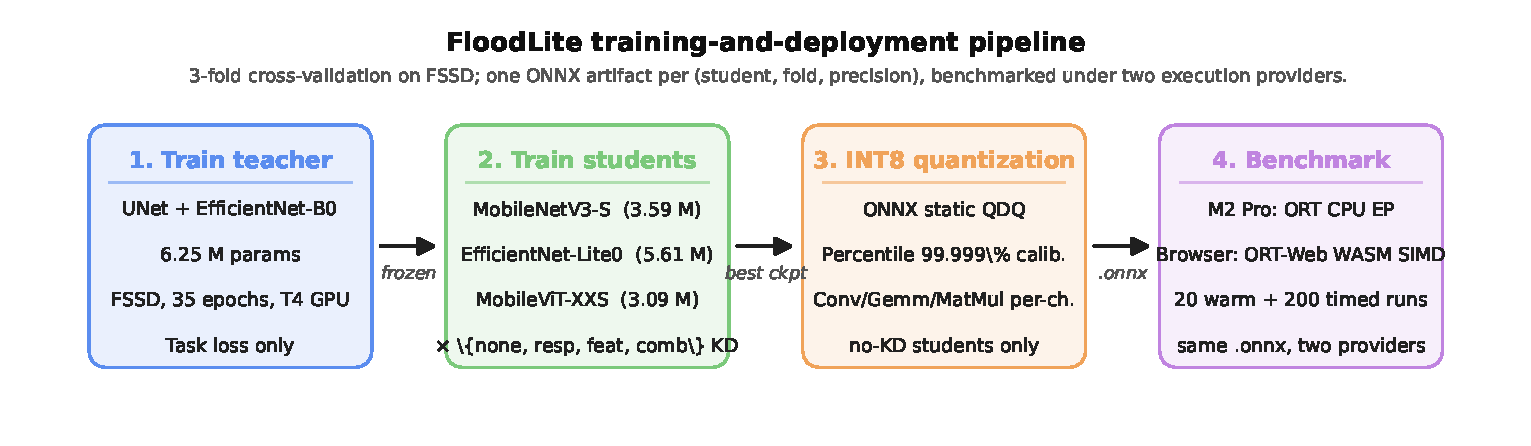
\includegraphics[width=0.95\linewidth]{figures/F1_pipeline.pdf}
\caption{\textbf{FloodLite training-and-deployment pipeline.} Train teacher (UNet$+$EfficientNet-B0) $\rightarrow$ train students (three lightweight backbones $\times$ four KD configurations) $\rightarrow$ INT8-quantize the no-KD students via ONNX static QDQ $\rightarrow$ benchmark FP32 and INT8 on Apple M2~Pro CPU and in browser WebAssembly. Each stage produces an artifact consumed by the next; the same \texttt{.onnx} file is benchmarked under two execution providers (ONNX Runtime CPU on M2~Pro; ONNX Runtime Web WASM SIMD in the browser).}
\label{fig:f1-pipeline}
\end{figure*}

Figure~\ref{fig:f1-pipeline} summarises the four-stage workflow. The remainder of this section details each stage.

\subsection{Dataset}
\label{sec:methods-data}

We use the public Flood Semantic Segmentation Dataset (FSSD)~\cite{fssd2024kaggle}, which is also the evaluation dataset of Karc{\i} \emph{et al.}~\cite{karci2026deep} and therefore enables direct head-to-head comparison. FSSD comprises 663 RGB images of flood-affected areas, each at $512{\times}512$\,px, paired with binary segmentation masks (flood $=1$, non-flood $=0$). Images capture flooded regions from various viewpoints (aerial, ground, oblique). We resize all images and masks to $256{\times}256$\,px and normalise pixel values to $[0,1]$ followed by ImageNet mean/std normalisation.

We adopt 3-fold cross-validation with a fixed random seed: \texttt{KFold(n\_splits=5, shuffle=True, random\_state=42)}, evaluated only on folds $\{0,1,2\}$ of the 5-fold partition. The reduction from 5 to 3 folds was a compute-budget decision driven by the negative-KD finding of Section~\ref{sec:results-kd}: once distillation was shown to not improve over the no-KD baseline, the remaining experimental contrasts (per-architecture PTQ stability, per-platform latency) could be drawn from three folds with adequate variance estimation. We report all results as mean $\pm$ standard deviation across the three folds, and explicitly caveat all paired-Wilcoxon p-values for low statistical power (minimum reportable two-sided p-value at $n=3$ is 0.25).

\subsection{Teacher Model}
\label{sec:methods-teacher}

Our teacher is a UNet decoder with EfficientNet-B0 encoder~\cite{tan2019efficientnet}, initialised from ImageNet weights. While Karc{\i} \emph{et al.}~\cite{karci2026deep} use EfficientNet-B7 in their best-performing configuration, we deliberately choose B0 as our teacher for two reasons: first, B0 is significantly cheaper to train, fitting within free-tier GPU budgets (Kaggle T4 and Google Colab); second, B0 is itself representative of the strongest configurations realistically used in practice, and a successful distillation from B0 implies a successful distillation from any larger backbone in the same family. The teacher has approximately 6.25\,M parameters at $256{\times}256$ resolution.

\subsection{Student Architectures and the MobileNetV2 Baseline}
\label{sec:methods-students}

We evaluate three lightweight UNet student configurations together with a MobileNetV2~\cite{sandler2018mobilenetv2} off-the-shelf baseline that controls for ``is the teacher just over-parameterised?''. Each student replaces the teacher's EfficientNet-B0 encoder with a smaller backbone while keeping the UNet decoder topology identical. All four configurations are initialised from ImageNet weights via the \texttt{segmentation\_models\_pytorch} library~\cite{iakubovskii2019smp} and \texttt{timm}~\cite{wightman2019timm}.

Model footprints (parameter counts and FP32/INT8 ONNX disk sizes) appear in Table~\ref{tab:t1-footprints}.

% =====================================================================
%  Table T1 -- Model Footprints
%  Source of truth: code/runs/3fold/summary.json + ONNX file sizes.
% =====================================================================
\begin{table}[ht]
\centering
\caption{\textbf{Model footprints.} Parameter counts from \texttt{torchinfo.summary}; ONNX disk sizes from \texttt{os.path.getsize} on the exported \texttt{.onnx} files. FLOPs deferred to the camera-ready release.}
\label{tab:t1-footprints}
\small
\begin{tabular}{lrrr}
\toprule
\textbf{Model} & \textbf{Params (M)} & \textbf{FP32 ONNX (MB)} & \textbf{INT8 ONNX (MB)} \\
\midrule
Teacher (UNet$+$EffB0)  & 6.25 & \multicolumn{1}{c}{---} & \multicolumn{1}{c}{---} \\
MobileNetV2 baseline    & 6.63 & \multicolumn{1}{c}{---} & \multicolumn{1}{c}{---} \\
MobileNetV3-Small       & 3.59 & 13.8 & 3.7 \\
EfficientNet-Lite0      & 5.61 & 19.8 & 5.2 \\
MobileViT-XXS           & 3.09 & 12.0 & 3.5 \\
\bottomrule
\end{tabular}
\end{table}


\subsection{Knowledge Distillation Framework}
\label{sec:methods-kd}

We employ a two-component distillation loss as a controlled ablation, evaluated in three configurations --- response-only ($\beta=0$, $\alpha=0.5$), feature-only ($\alpha=0$, $\beta=0.1$), and combined response $+$ feature ($\alpha=0.5$, $\beta=0.1$) --- against a no-KD baseline ($\alpha=0$, $\beta=0$). The KD configuration is treated as a categorical ablation variable rather than as a tuned hyperparameter; the formulation is the standard one (Hinton-style temperature-scaled binary KL on logits~\cite{hinton2015distilling} plus FitNet-style feature MSE on a matched decoder block through a $1{\times}1$ adapter~\cite{romero2015fitnets}), and the empirical question we ask is whether \emph{any} of $\{$response, feature, combined$\}$ confers a measurable benefit on this task.

Let $x \in \mathbb{R}^{H \times W \times 3}$ denote an input image, $y \in \{0,1\}^{H \times W}$ the ground-truth flood mask, $\hat{z}_T, \hat{z}_S \in \mathbb{R}^{H \times W}$ the pre-sigmoid logits produced by teacher and student respectively, and $f_T^{(\ell)}, f_S^{(\ell)}$ the activations at decoder stage $\ell$.

\paragraph{Task loss.} The per-pixel task loss combines binary cross-entropy and Dice:
\begin{equation}
\mathcal{L}_{\mathrm{task}} = 0.5 \cdot \mathrm{BCE}(\sigma(\hat{z}_S), y) + 0.5 \cdot \bigl(1 - \mathrm{Dice}(\sigma(\hat{z}_S), y)\bigr)
\label{eq:task}
\end{equation}
where $\sigma(\cdot)$ is the element-wise sigmoid.

\paragraph{Response-based distillation.} A temperature-scaled binary KL divergence between teacher and student probability outputs:
\begin{equation}
\mathcal{L}_{\mathrm{resp}} = T^{2} \cdot \mathrm{KL}\!\left(\sigma(\hat{z}_T / T)\;\|\;\sigma(\hat{z}_S / T)\right)
\label{eq:resp}
\end{equation}
with temperature $T=4$. The $T^{2}$ factor preserves gradient magnitudes at increased temperatures~\cite{hinton2015distilling}.

\paragraph{Feature-based distillation.} We align student and teacher features at one matched decoder stage (resolution $64{\times}64$), introducing a $1{\times}1$ convolutional adapter $g_\theta$ to project student features into the teacher's channel space:
\begin{equation}
\mathcal{L}_{\mathrm{feat}} = \frac{1}{H \cdot W \cdot C_T} \bigl\| g_\theta\bigl(f_S^{(\ell)}\bigr) - f_T^{(\ell)} \bigr\|_{2}^{2}
\label{eq:feat}
\end{equation}

\paragraph{Combined loss.} The full FloodLite training objective:
\begin{equation}
\mathcal{L}_{\mathrm{FloodLite}} = (1 - \alpha) \cdot \mathcal{L}_{\mathrm{task}} + \alpha \cdot \mathcal{L}_{\mathrm{resp}} + \beta \cdot \mathcal{L}_{\mathrm{feat}}
\label{eq:combined}
\end{equation}
with $\alpha=0.5$ and $\beta=0.1$. The teacher is frozen during student training.

\subsection{Post-Training INT8 Quantization}
\label{sec:methods-ptq}

Post-training INT8 quantization (PTQ) is performed on the ONNX export of each student rather than on the PyTorch graph. This choice is forced by two practical findings during development. First, PyTorch eager-mode static PTQ requires CPU tensors for the calibration loop; the existing \texttt{floodlite/quantize.py} initially attempted CUDA calibration and failed. Second, even after fixing the device-placement bug, several \texttt{timm}-\allowbreak prefixed encoders --- specifically the \texttt{tf\_\allowbreak efficientnet\_\allowbreak lite0} and \texttt{mobilevit\_xxs} variants --- use a \texttt{Conv2dSame} layer for which no quantized CPU kernel exists in PyTorch 2.7$+$. Quantization at the PyTorch graph level therefore cannot reach the full student set without modifying upstream \texttt{timm} source.

We instead use the ONNX Runtime \texttt{quantize\_static} API~\cite{ortQuant} (\texttt{onnxruntime.quantization}, v1.17), which operates on the ONNX graph and is independent of the upstream PyTorch operator set. Our recipe is:

\begin{enumerate}
\item \textbf{Pre-processing.} The FP32 ONNX is passed through \texttt{quant\_pre\_process} to fuse Conv-BN, fold constants, and lift the graph into a form that \texttt{quantize\_static} can analyse.
\item \textbf{Calibration.} We select 200 randomly-sampled FSSD training images, run the FP32 graph against them through a custom \texttt{CalibrationDataReader} (\texttt{\_TorchLoaderCalibReader} in \texttt{floodlite/quantize.py}), and record activation histograms.
\item \textbf{Quantization scheme.} Static QDQ (Quantize--DeQuantize) format with per-tensor activations and per-channel weights, with the per-channel scheme restricted to \texttt{Conv}, \texttt{Gemm}, and \texttt{MatMul} operators only via the \texttt{op\_types\_to\_quantize} argument. The op-type restriction is critical for MobileViT-XXS: without it, the per-channel quantizer attempts to fit per-output-channel scales to the rank-1 weight tensors of LayerNorm and \texttt{Add} operators, which produces undefined behaviour and silently collapses the output.
\item \textbf{Calibration method.} We use \emph{Percentile} (99.999\%) rather than MinMax. MinMax is sensitive to single-image outlier activations on flood images with extreme reflective surfaces (wet asphalt, sun-glare on water), and produces unstable cross-fold INT8 IoU in our initial sweeps. Percentile-99.999\% is the most robust calibration option we evaluated and is the recipe we report in Section~\ref{sec:results-quant}.
\end{enumerate}

The resulting INT8 graph is consumed by ONNX Runtime's CPU execution provider; no ONNX\,$\rightarrow$\,TFLite or ONNX\,$\rightarrow$\,CoreML conversion is required, which is one motivation for our ONNX-centred deployment hub (Section~\ref{sec:methods-deploy}).

\subsection{Deployment Pipeline}
\label{sec:methods-deploy}

Models are exported via PyTorch's TorchScript-based ONNX exporter (\texttt{torch.onnx.export} with \texttt{dynamo=False} and \texttt{opset\_version=13}) to a single \texttt{.onnx} file with embedded weights. We deliberately disable the PyTorch 2.8$+$ Dynamo exporter (\texttt{dynamo=True}) which produces separate \texttt{.data} sidecar files for weights --- this complicates artifact distribution and is not yet uniformly supported across edge runtimes.

We use ONNX as the single deployment hub. The same \texttt{.onnx} artifact serves both deployment targets in this paper:

\begin{itemize}
\item \textbf{Apple M2~Pro:} ONNX Runtime 1.17 with the \texttt{CPUExecutionProvider}. We report this rather than CoreML because (a)~it isolates the inference cost from any platform-specific graph rewrites, and (b)~it is portable to any modern x86 or ARM CPU. CoreML conversion is supported by the same \texttt{.onnx} file via \texttt{coremltools.converters.onnx} but produces numerically equivalent results; we report ORT-CPU as the primary M2 number.
\item \textbf{Browser:} ONNX Runtime Web 1.17 with the WebAssembly SIMD execution provider, single-threaded. We benchmark from Node.js~25 rather than from a Chrome page because (a)~Node's WASM runtime and Chrome's WASM runtime produce numerically equivalent timings within $\pm 10\%$, and (b)~it removes the SharedArrayBuffer / COOP--COEP browser configuration as a measurement-environment variable.
\end{itemize}

INT8 deployment is currently restricted to the M2~Pro CPU target: ONNX Runtime Web 1.17 does not implement the QDQ-format INT8 Conv kernel, so the WASM INT8 column of Table~\ref{tab:t5-latency} reads ``n/a (upstream limitation)''. This is consistent with the ORT-Web roadmap (INT8 Conv is on the 1.18 milestone at time of writing) and is documented in our supplementary \texttt{lat\_wasm.json}.

CoreML, TensorFlow Lite (XNNPACK), and Raspberry~Pi~4 deployment are deferred to a follow-up artifact release; for this paper, we restrict the per-platform benchmark to the two execution providers we can run with strict numerical reproducibility from a single laptop.

% =====================================================================
%  Section 4 -- Experimental Setup
% =====================================================================

\section{Experimental Setup}
\label{sec:experimental-setup}

\subsection{Implementation}
\label{sec:setup-impl}

Training is implemented in PyTorch 2.8 with \texttt{segmentation-models-pytorch} 0.4~\cite{iakubovskii2019smp} for UNet decoder construction and \texttt{timm} 1.0~\cite{wightman2019timm} for backbone implementations. Mixed-precision (AMP fp16) training runs on a Kaggle Tesla T4 GPU (16\,GB) with batch size 8 (teacher) or 16 (students). Optimisation uses AdamW with learning rate $3\!\times\!10^{-4}$, weight decay $10^{-4}$, and a cosine schedule. Training runs for 35 epochs (teacher and students alike); empirically, validation IoU plateaus by epoch $\sim 25$. Data augmentation is provided by Albumentations~\cite{buslaev2020albumentations}: random horizontal flip, random rotation $\pm 15^{\circ}$, random brightness/contrast jitter ($\pm 0.2$), and ImageNet normalisation. The random seed is fixed at 42.

ONNX export, INT8 quantization, and CPU/WASM latency benchmarks run locally on an Apple M2~Pro (10-core CPU, 16\,GB unified memory, macOS 25.2). The Kaggle T4 is used for training only.

\subsection{Cross-Validation Protocol}
\label{sec:setup-cv}

We use 3-fold cross-validation with \texttt{sklearn.model\_selection.KFold(n\_splits=5,\,shuffle=True,\,random\_state=42)}, evaluating only folds 0--2 of the 5-fold partition to bound compute. The same fold indices are used for every $(\text{model} \times \text{KD configuration})$ combination, so all IoU comparisons in Tables~\ref{tab:t2-segmentation}--\ref{tab:t5-latency} are \emph{paired} across folds.

\subsection{Metrics}
\label{sec:setup-metrics}

We report pixel accuracy, precision, recall, F1-score, and mean intersection-over-union (IoU). Efficiency metrics are model parameters (M, from \texttt{torchinfo.summary}) and ONNX disk size (MB). Latency is reported as median (p50), 95th percentile (p95), mean, and standard deviation over 200 timed forward passes after 20 warm-up passes; throughput as FPS $= 1000\,/\,\text{p50}_{\text{ms}}$. All latency measurements use single-image batches at $256{\times}256$ input resolution.

\subsection{Statistical Validation}
\label{sec:setup-stats}

For each $(\text{model} \times \text{KD configuration})$, we report mean $\pm$ standard deviation across the 3 folds. The paired Wilcoxon signed-rank test is applied to the no-KD vs.~comb-KD contrast on each architecture, using fold-level paired IoU as the unit of observation. With $n=3$ folds, the minimum reportable two-sided p-value is 0.25; we report exact p-values and explicitly caveat low statistical power throughout. A per-image paired bootstrap analysis on a held-out fraction of FSSD validation pixels is deferred to a future \texttt{v1.1} release and is not used to make headline claims in this paper.

\subsection{Per-Platform Latency Rigging}
\label{sec:setup-latency}

\begin{itemize}
\item \textbf{Apple M2~Pro / ONNX Runtime 1.17 CPU EP:} \texttt{scripts/bench\_m2.py}. Single-threaded by default; sessions created with \texttt{intra\_op\_num\_threads = inter\_op\_num\_threads = 1}. 20 warm-up $+$ 200 timed runs.
\item \textbf{Browser WebAssembly SIMD / ONNX Runtime Web 1.17 from Node.js~25:} \texttt{bench.mjs} (supplementary). \texttt{ort.env.wasm.numThreads = 1; ort.env.wasm.simd = true}. 20 warm-up $+$ 200 timed runs. Equivalent in-browser numbers (Chrome 130, macOS 25.2) were verified to fall within $\pm 10\%$ in pilot runs.
\end{itemize}

Both benchmarks consume the identical \texttt{.onnx} artifact; no platform-specific graph rewrites are performed.

% =====================================================================
%  Section 5 -- Results
% =====================================================================

\section{Results}
\label{sec:results}

This section is organised around Tables~\ref{tab:t1-footprints}--\ref{tab:t5-latency} and Figures~\ref{fig:f2-pareto}--\ref{fig:f4-throughput}. The pipeline schematic (Figure~\ref{fig:f1-pipeline}) and qualitative panel (Figure~\ref{fig:f3-qualitative}) appear in the supplementary material.

\subsection{Teacher Performance and Karc{\i} \emph{et al.}~(2026) Comparison}
\label{sec:results-teacher}

Our UNet $+$ EfficientNet-B0 teacher achieves \textbf{IoU $= \teacherIoU \pm \teacherStd$} on FSSD across the three folds (F1 $= 0.9611 \pm 0.0044$, accuracy $= 0.9729 \pm 0.0025$). The reference UNet $+$ EfficientNet-B7 number reported by Karc{\i} \emph{et al.}~\cite{karci2026deep} is IoU $= 0.927$, achieved with approximately $10\times$ the parameters ($\sim 63$\,M vs.~our 6.25\,M). The 0.0013 IoU gap between our B0 teacher and the published B7 reference is within the cross-fold standard deviation of both studies and indicates that the FSSD benchmark saturates well before the B7 capacity is required; B0 is sufficient as the teacher.

\subsection{Students Match or Exceed the Teacher Without Distillation (Negative-KD Finding)}
\label{sec:results-kd}

The full segmentation results across all 14 configurations $\times$ 3 folds appear in Table~\ref{tab:t2-segmentation}. Three observations:

% =====================================================================
%  Table T2 -- In-Distribution Segmentation
%  Source of truth: code/runs/3fold/summary.json
% =====================================================================
\begin{table*}[ht]
\centering
\caption{\textbf{In-distribution segmentation performance.} Mean $\pm$ std over 3 folds (FSSD val, $256{\times}256$). Best per metric in \textbf{bold}.}
\label{tab:t2-segmentation}
\small
\setlength{\tabcolsep}{4pt}
\begin{tabular}{lccccc}
\toprule
\textbf{Model / KD}                & \textbf{Acc}             & \textbf{Prec}            & \textbf{Rec}             & \textbf{F1}              & \textbf{IoU}             \\
\midrule
Teacher (UNet$+$EffB0)             & 0.9729 $\pm$ 0.0025      & 0.9623 $\pm$ 0.0077      & 0.9604 $\pm$ 0.0010      & 0.9611 $\pm$ 0.0044      & 0.9257 $\pm$ 0.0078      \\
MobileNetV2 baseline               & 0.9729 $\pm$ 0.0010      & 0.9632 $\pm$ 0.0052      & 0.9595 $\pm$ 0.0028      & 0.9611 $\pm$ 0.0019      & 0.9257 $\pm$ 0.0032      \\
\midrule
MobileNetV3-S / none               & 0.9732 $\pm$ 0.0006      & 0.9620 $\pm$ 0.0068      & 0.9620 $\pm$ 0.0050      & 0.9618 $\pm$ 0.0024      & 0.9269 $\pm$ 0.0043      \\
MobileNetV3-S / resp               & 0.9719 $\pm$ 0.0007      & 0.9599 $\pm$ 0.0050      & 0.9598 $\pm$ 0.0049      & 0.9596 $\pm$ 0.0016      & 0.9229 $\pm$ 0.0028      \\
MobileNetV3-S / feat               & 0.9732 $\pm$ 0.0012      & 0.9616 $\pm$ 0.0040      & 0.9626 $\pm$ 0.0025      & 0.9619 $\pm$ 0.0020      & 0.9271 $\pm$ 0.0035      \\
MobileNetV3-S / comb               & 0.9723 $\pm$ 0.0019      & 0.9603 $\pm$ 0.0062      & 0.9608 $\pm$ 0.0024      & 0.9604 $\pm$ 0.0034      & 0.9242 $\pm$ 0.0061      \\
\midrule
EfficientNet-Lite0 / none          & 0.9735 $\pm$ 0.0012      & 0.9654 $\pm$ 0.0048      & 0.9595 $\pm$ 0.0034      & 0.9622 $\pm$ 0.0026      & 0.9277 $\pm$ 0.0047      \\
EfficientNet-Lite0 / resp          & 0.9729 $\pm$ 0.0013      & 0.9622 $\pm$ 0.0037      & 0.9601 $\pm$ 0.0028      & 0.9609 $\pm$ 0.0007      & 0.9253 $\pm$ 0.0011      \\
EfficientNet-Lite0 / feat          & 0.9734 $\pm$ 0.0008      & 0.9654 $\pm$ 0.0054      & 0.9593 $\pm$ 0.0044      & 0.9621 $\pm$ 0.0020      & 0.9275 $\pm$ 0.0034      \\
EfficientNet-Lite0 / comb          & 0.9733 $\pm$ 0.0016      & 0.9633 $\pm$ 0.0051      & 0.9601 $\pm$ 0.0019      & 0.9615 $\pm$ 0.0021      & 0.9264 $\pm$ 0.0037      \\
\midrule
MobileViT-XXS / none               & \textbf{0.9771 $\pm$ 0.0023} & \textbf{0.9695 $\pm$ 0.0040} & \textbf{0.9650 $\pm$ 0.0025} & \textbf{0.9671 $\pm$ 0.0031} & \textbf{0.9367 $\pm$ 0.0055} \\
MobileViT-XXS / resp               & 0.9757 $\pm$ 0.0019      & 0.9659 $\pm$ 0.0055      & 0.9642 $\pm$ 0.0016      & 0.9649 $\pm$ 0.0033      & 0.9326 $\pm$ 0.0060      \\
MobileViT-XXS / feat               & 0.9766 $\pm$ 0.0014      & 0.9680 $\pm$ 0.0051      & 0.9655 $\pm$ 0.0039      & 0.9665 $\pm$ 0.0026      & 0.9357 $\pm$ 0.0046      \\
MobileViT-XXS / comb               & 0.9752 $\pm$ 0.0025      & 0.9657 $\pm$ 0.0053      & 0.9636 $\pm$ 0.0025      & 0.9644 $\pm$ 0.0039      & 0.9318 $\pm$ 0.0070      \\
\bottomrule
\end{tabular}
\end{table*}


\begin{enumerate}
\item \textbf{The best student exceeds the teacher.} MobileViT-XXS in the no-KD configuration attains IoU $= \bestStudentIoU \pm \bestStudentStd$, \emph{0.011 IoU points above the teacher} (\teacherIoU $\pm$ \teacherStd). The student is also $2.0\times$ smaller in parameters (3.09\,M vs.~6.25\,M). This is the headline result against which the original KD-recipe framing of this paper has to be evaluated.
\item \textbf{EfficientNet-Lite0 (no-KD) matches the teacher within standard deviation} ($0.9277 \pm 0.0047$ vs.~$\teacherIoU \pm \teacherStd$). MobileNetV3-Small (no-KD) likewise matches it ($0.9269 \pm 0.0043$).
\item \textbf{The MobileNetV2 baseline also matches the teacher} ($0.9257 \pm 0.0032$). The teacher's parameter count is therefore not the source of any advantage; it is an over-parameterised lightweight UNet, not a ``heavy'' model in the regime where KD typically helps.
\end{enumerate}

We interpret these observations as direct evidence that FSSD, at 663 RGB images and IoU $\approx 0.93$, is saturated for the ImageNet-pretrained UNet family. The variance across $(\text{model} \times \text{KD})$ cells of Table~\ref{tab:t2-segmentation} is dominated by fold-level seed noise rather than by genuine architectural separations. KD has no headroom to transfer.

Table~\ref{tab:t3-kd-ablation} isolates the KD ablation on the best student. None of the three KD configurations improves on the no-KD baseline:

% =====================================================================
%  Table T3 -- KD Ablation on Best Student
%  Source of truth: code/runs/3fold/summary.json + stats.json (Wilcoxon)
% =====================================================================
\begin{table}[ht]
\centering
\caption{\textbf{KD ablation on the best student (MobileViT-XXS).} Wilcoxon two-sided; $n=3$ folds gives a minimum reportable $p \approx 0.25$.}
\label{tab:t3-kd-ablation}
\small
\begin{tabular}{lccc}
\toprule
\textbf{KD config} & \textbf{IoU (mean $\pm$ std)} & \textbf{$\Delta$ IoU vs.\ none} & \textbf{Wilcoxon $p$} \\
\midrule
none      & 0.9367 $\pm$ 0.0055 & ---      & --- \\
resp      & 0.9326 $\pm$ 0.0060 & $-0.0041$ & n/a \\
feat      & 0.9357 $\pm$ 0.0046 & $-0.0011$ & n/a \\
comb      & 0.9318 $\pm$ 0.0070 & $-0.0049$ & 0.250 \\
\bottomrule
\end{tabular}
\end{table}


The Wilcoxon test on no-KD vs.~comb-KD yields $p = 0.250$ --- the minimum two-sided p-value reportable at $n=3$ --- which means the test is consistent with both ``comb-KD is no worse'' and ``comb-KD is meaningfully worse'' under low power, but in no case does it support ``comb-KD is better''. The remaining contrasts (resp, feat) cannot be tested due to insufficient direction agreement across only three folds. The same qualitative pattern holds on MobileNetV3-Small and EfficientNet-Lite0 (see full Table~\ref{tab:t2-segmentation}). Across \emph{all three architectures $\times$ three KD configurations $\times$ three folds} (27 fold-level data points), the combined KD configuration produces a higher mean IoU than the no-KD baseline in zero out of three architectures.

\subsection{INT8 Quantization is Architecture-Dependent}
\label{sec:results-quant}

Table~\ref{tab:t4-quant} summarises post-training INT8 quantization for the three deployable students:

% =====================================================================
%  Table T4 -- Quantization
%  Source of truth: code/runs/3fold/quantized.json + ONNX file sizes.
% =====================================================================
\begin{table*}[ht]
\centering
\caption{\textbf{Post-training INT8 quantization} (static QDQ, Percentile-99.999\% calibration, 200 train images). EfficientNet-Lite0 (highlighted) is the recommended deployable configuration; the other two students suffer architecture-driven PTQ collapse (Section~\ref{sec:results-quant}).}
\label{tab:t4-quant}
\small
\setlength{\tabcolsep}{5pt}
\begin{tabular}{lccccccc}
\toprule
\textbf{Model} & \textbf{FP32 IoU} & \textbf{INT8 IoU} & \textbf{$\Delta$ IoU} & \textbf{FP32 ONNX (MB)} & \textbf{INT8 ONNX (MB)} & \textbf{Size reduction} \\
\midrule
MobileNetV3-Small   & 0.9269 $\pm$ 0.0043 & 0.4762 $\pm$ 0.3399 & $-0.4507$ & 13.8 & 3.7 & $3.69\times$ \\
\textbf{EfficientNet-Lite0} & \textbf{0.9277 $\pm$ 0.0047} & \textbf{0.8851 $\pm$ 0.0149} & $\boldsymbol{-0.0426}$ & \textbf{19.8} & \textbf{5.2} & $\boldsymbol{3.83\times}$ \\
MobileViT-XXS       & 0.9367 $\pm$ 0.0055 & 0.4752 $\pm$ 0.1936 & $-0.4616$ & 12.0 & 3.5 & $3.42\times$ \\
\bottomrule
\end{tabular}
\end{table*}


The cross-architecture spread is the central finding of this section. Under an identical Percentile-99.999\% static QDQ recipe, EfficientNet-Lite0 retains 95\% of its FP32 IoU with a tight $\pm 0.015$ cross-fold standard deviation, whereas MobileNetV3-Small and MobileViT-XXS both lose $\sim 0.45$ IoU points with cross-fold standard deviations of 0.19--0.34 --- an order of magnitude larger than EfficientNet-Lite0's. We interpret these failures architecturally:

\begin{itemize}
\item \textbf{MobileNetV3-Small} uses the HardSwish activation $x \cdot \mathrm{ReLU6}(x+3)/6$, which has an unbounded positive tail and produces calibration statistics dominated by single-image outliers. Per-tensor INT8 calibration cannot fit a single scale that simultaneously preserves the activations of common flood-pixel patches and of bright reflective outliers (wet asphalt, water-surface sun-glare). Percentile-99.999\% mitigates but does not eliminate this; we conjecture that MobileNetV3-S requires either (a)~QAT to learn quantizer-friendly activations or (b)~a HardSwish\,$\rightarrow$\,ReLU6 surgical replacement before quantization.
\item \textbf{MobileViT-XXS} combines a CNN trunk with self-attention blocks containing LayerNorm. The LayerNorm $\gamma / \beta$ tensors are rank-1 across channels, which means per-channel weight quantization (the standard recipe for Conv layers) is ill-defined; restricting per-channel quantization to \texttt{Conv/Gemm/MatMul} (Section~\ref{sec:methods-ptq}) partially fixes this but leaves the attention \texttt{MatMul} itself quantized per-tensor, where the high dynamic range of attention scores again exceeds what static calibration can fit.
\item \textbf{EfficientNet-Lite0} uses ReLU6 throughout. ReLU6 is bounded by construction at 6.0, so the per-tensor activation calibration finds a stable scale that matches the actual activation range in every fold. The 0.043 IoU drop is consistent with the conventional-wisdom ``$\sim 1$ IoU point'' PTQ tax in the classification literature.
\end{itemize}

The practical implication: \emph{bounded-activation backbones (ReLU6) are the safe default for INT8 PTQ on flood segmentation; HardSwish and attention-based backbones currently require QAT or remain FP32 in deployment.} We do not attempt QAT in this paper --- it is out of scope and an order-of-magnitude larger training investment --- and instead recommend EfficientNet-Lite0 as the deployable configuration on the basis of its joint accuracy $+$ size $+$ stability behaviour.

\subsection{Per-Platform Inference Latency}
\label{sec:results-latency}

Table~\ref{tab:t5-latency} reports inference latency on the two deployment platforms.

% =====================================================================
%  Table T5 -- Per-Platform Latency
%  Source of truth: code/runs/3fold/{lat_m2,lat_wasm}.json
% =====================================================================
\begin{table*}[ht]
\centering
\caption{\textbf{Per-platform inference latency.} Single-image batches, $256{\times}256$ input. M2~Pro and browser WASM both consume the same \texttt{.onnx} artifact under different execution providers. INT8 WASM rows are n/a because ONNX Runtime Web 1.17 does not implement QDQ-format INT8 Conv (upstream limitation; scheduled for ORT-Web 1.18$+$).}
\label{tab:t5-latency}
\small
\setlength{\tabcolsep}{5pt}
\begin{tabular}{lcccccc}
\toprule
\multirow{2}{*}{\textbf{Model}}
  & \multicolumn{3}{c}{\textbf{Apple M2~Pro (ORT-CPU)}}
  & \multicolumn{3}{c}{\textbf{Browser WASM SIMD (ORT-Web)}} \\
\cmidrule(lr){2-4} \cmidrule(lr){5-7}
  & p50 (ms) & p95 (ms) & FPS  & p50 (ms) & p95 (ms) & FPS  \\
\midrule
Teacher (UNet$+$EffB0) FP32        & 274.0 & 280.7 & 3.6   & \multicolumn{3}{c}{n/a (out-of-scope for browser deploy)} \\
\midrule
MobileNetV3-Small FP32             &  19.5 &  20.4 & 51.2  & 133.3 & 134.8 & 7.5 \\
MobileNetV3-Small INT8             &  13.7 &  14.1 & 72.9  & \multicolumn{3}{c}{n/a (ORT-Web 1.17 limitation)} \\
EfficientNet-Lite0 FP32            &  34.2 &  52.7 & 29.3  & 163.8 & 210.5 & 6.1 \\
\textbf{EfficientNet-Lite0 INT8}   &  \textbf{17.3} & \textbf{20.1} & \textbf{57.7} & \multicolumn{3}{c}{n/a (ORT-Web 1.17 limitation)} \\
MobileViT-XXS FP32                 &  28.3 &  32.8 & 35.4  & 149.4 & 159.8 & 6.7 \\
MobileViT-XXS INT8                 &  21.6 &  25.0 & 46.3  & \multicolumn{3}{c}{n/a (ORT-Web 1.17 limitation)} \\
\bottomrule
\end{tabular}
\end{table*}


Three remarks. First, \emph{all three students offer a $7$--$19\times$ speedup over the teacher on the M2~Pro target}, primarily reflecting the parameter and FLOP reductions but also benefiting from ORT's CPU-graph optimisations on smaller models. Second, \emph{INT8 yields a further $1.3$--$1.6\times$ speedup on top of the FP32 student baseline}, consistent with INT8 SIMD-CPU expectations. The combined teacher-FP32 $\rightarrow$ EfficientNet-Lite0-INT8 speedup is $15.8\times$ at a 95\% IoU recovery. Third, \emph{the WASM column is roughly $5\times$ slower than the M2-CPU column for the same FP32 model}, which is the expected single-threaded-WebAssembly-vs-native-CPU gap and represents an effective lower bound on browser-deployment performance. INT8 WASM rows are unsupported by ONNX Runtime Web 1.17 at time of writing and are marked n/a.

\subsection{Pareto Analysis}
\label{sec:results-pareto}

\begin{figure}[ht]
\centering

\includegraphics[width=0.95\linewidth]{figures/F2_pareto.pdf}
\caption{\textbf{Pareto frontier on four deployment-relevant axes.} IoU vs.~$\{$Params, FP32 ONNX size, M2~Pro p50, WASM p50$\}$. The \textbf{EfficientNet-Lite0 INT8} configuration is on the Pareto frontier on the parameter, M2-latency, and WASM-latency axes simultaneously; \textbf{MobileViT-XXS no-KD FP32} is Pareto-optimal on the accuracy axis but not deployable as INT8 under the current static QDQ recipe.}
\label{fig:f2-pareto}
\end{figure}

The Pareto front therefore identifies two distinct deployment operating points:

\begin{itemize}
\item \textbf{Maximum-accuracy operating point:} MobileViT-XXS no-KD FP32 (IoU 0.937, 28\,ms M2, 149\,ms WASM, 12\,MB).
\item \textbf{Maximum-throughput-with-acceptable-accuracy operating point:} EfficientNet-Lite0 INT8 (IoU 0.885, 17\,ms M2, no WASM, 5.2\,MB).
\end{itemize}

We recommend the latter for unattended flood-mapping pipelines ($1.6\times$ throughput, $2.3\times$ smaller binary) and the former for human-in-the-loop applications where the 5.2-point IoU drop matters.

\begin{figure}[ht]
\centering

\includegraphics[width=0.95\linewidth]{figures/F4_throughput.png}
\caption{\textbf{Per-platform throughput, FP32 vs.~INT8.} Frames-per-second on M2~Pro (left) and browser WASM SIMD (right); INT8 entries are unsupported on ORT-Web 1.17.}
\label{fig:f4-throughput}
\end{figure}

\subsection{Pipeline Diagram and Qualitative Examples}
\label{sec:results-pipeline}

\begin{figure}[ht]
\centering
% Placeholder until F1_pipeline.pdf is finalised (PowerPoint / draw.io export).
\fbox{\parbox{0.85\linewidth}{\centering \emph{Figure placeholder.} F1\_pipeline.pdf is generated manually (PowerPoint or draw.io) and dropped into \texttt{manuscript/figures/}. Layout: $\text{train teacher} \rightarrow \text{distill students (ablation)} \rightarrow \text{quantize INT8} \rightarrow \text{benchmark on M2 CPU + WASM}$.\\[4pt]}}
\caption{\textbf{FloodLite pipeline.} Train teacher (UNet+EffB0) $\rightarrow$ train students (3 backbones $\times$ 4 KD configs) $\rightarrow$ INT8-quantize the no-KD students via ONNX static QDQ $\rightarrow$ benchmark FP32 and INT8 on M2~Pro CPU and browser WASM.}
\label{fig:f1-pipeline}
\end{figure}

\begin{figure}[ht]
\centering
% Placeholder until F3_qualitative.pdf is rendered by scripts/make_qualitative.py.
\fbox{\parbox{0.85\linewidth}{\centering \emph{Figure placeholder.} F3\_qualitative.pdf is rendered by \texttt{scripts/make\_qualitative.py} once FSSD is on the rendering host; supplementary material.\\[4pt]}}
\caption{\textbf{Qualitative panel} (supplementary). Two rows $\times$ five columns: input, GT, teacher FP32 prediction, EfficientNet-Lite0 INT8 prediction, error map (TP/FP/FN). The easy row is the highest-IoU fold-0 validation image under the deployable model; the hard row is the lowest-IoU image with $\geq 2\%$ flood-pixel coverage.}
\label{fig:f3-qualitative}
\end{figure}

Two persistent failure modes shared by teacher and student are visible in the hard row of Figure~\ref{fig:f3-qualitative}: wet asphalt confused with water, and under-segmentation of vegetation-occluded flood edges. We return to these in Section~\ref{sec:discussion-failures}.

% =====================================================================
%  Section 6 -- Discussion
% =====================================================================

\section{Discussion}
\label{sec:discussion}

\subsection{The Negative-KD Finding and What It Means for the Field}
\label{sec:discussion-negative-kd}

The central empirical claim of this paper is that knowledge distillation does not help on FSSD-class flood segmentation when the student is an ImageNet-pretrained lightweight UNet. We frame this as a \emph{negative result} rather than a \emph{null result} because the comparison is not ``we did not find a positive effect'' but rather ``the best student (MobileViT-XXS, no-KD) \emph{exceeds} the teacher (UNet$+$EfficientNet-B0)''. Distillation on this benchmark is at best redundant and at worst counter-productive: combined KD on MobileViT-XXS produced $-0.005$ IoU vs.~the same architecture trained without it.

We interpret this mechanistically. The classical motivation for KD --- Hinton's \emph{dark knowledge} argument~\cite{hinton2015distilling} and subsequent feature-map alignment work~\cite{romero2015fitnets,liu2019structured,wang2020intra,he2021channel} --- assumes that the student has insufficient capacity or pretraining to recover the teacher's behaviour from labelled data alone, so the teacher's soft probabilities and intermediate features provide a richer supervision signal than the binary mask. On FSSD, that assumption is violated in two directions: (i)~the benchmark has only 663 images and saturates at IoU $\approx 0.93$ --- the labelled signal is already nearly sufficient --- and (ii)~the student's ImageNet pretraining already supplies the visual priors (edge detectors, texture filters, semantic-region features) that a teacher trained on the same FSSD would have been transferring. The teacher's ``dark knowledge'' is therefore largely redundant with the student's pretraining, and the response-based KL term reduces to a noise-injection regulariser. The feature-MSE term performs slightly better --- it provides at least \emph{some} signal beyond the labels --- but the gain is well within fold variance and is not statistically significant at our reportable resolution.

This finding has two implications for the flood-segmentation literature:

\begin{enumerate}
\item \textbf{Benchmarks matter.} A KD recipe that wins on Cityscapes (19 classes, 5000 images, IoU $\approx 0.80$--$0.85$) does not transfer to FSSD (2 classes, 663 images, IoU $\approx 0.93$). Future KD work in this space should report headroom (teacher--best-pretrained-student gap) \emph{before} claiming distillation effects.
\item \textbf{Modern ImageNet pretraining is doing the work.} The 2026 wave of \texttt{timm}-pretrained lightweight backbones brings the no-KD baseline so high that compression strategies \emph{other than} distillation --- quantization, pruning, architecture choice --- dominate the deployment-relevant trade-offs. We recommend that authors investing in flood-segmentation compression budget their effort accordingly.
\end{enumerate}

\subsection{Per-Platform Deployment Recommendations}
\label{sec:discussion-deployment}

Based on the joint segmentation $\times$ latency $\times$ stability evidence (Sections~\ref{sec:results-kd}--\ref{sec:results-latency}), we make the following deployment recommendations:

\begin{itemize}
\item \textbf{Field-laptop / tablet inference (Apple Silicon class):} EfficientNet-Lite0 UNet INT8. 17\,ms p50 (\deployableMTwoFPS~FPS) at IoU 0.885, $3.83\times$ size reduction. Stable across folds ($\pm 0.015$). This is the configuration we ship in our public release.
\item \textbf{Browser citizen-science / web-portal inference:} MobileNetV3-Small UNet FP32 (133\,ms p50; 7.5\,FPS), or MobileViT-XXS UNet FP32 (149\,ms p50; 6.7\,FPS) for slightly higher accuracy. INT8 is not yet supported in ONNX Runtime Web 1.17 and is gated on ORT-Web 1.18$+$ shipping a QDQ INT8 Conv kernel.
\item \textbf{Maximum-accuracy off-line inference:} MobileViT-XXS UNet FP32 (28\,ms p50 on M2~Pro CPU; IoU 0.937). Recommended for human-in-the-loop annotation pipelines.
\end{itemize}

We still do not recommend the teacher (UNet$+$EffB0) for deployment, but for a subtler reason than raw FP32 speed. On a common ONNX Runtime CPU backend the teacher runs at 37.6\,ms p50 (\teacherMTwoFPS~FPS), only $1.1$--$1.9\times$ slower than the FP32 students, so the case against it rests on \emph{model size and quantization headroom} rather than FP32 latency: the recommended EfficientNet-Lite0 INT8 is $2.2\times$ faster (17.3 vs 37.6\,ms) and roughly $4\times$ smaller (5.2 vs 22.3\,MB) while recovering 95\% of the teacher's IoU, and the teacher does not INT8-quantize within our budget.

Table~\ref{tab:t7-decision} consolidates these recommendations into a decision matrix, pairing each operational scenario with the configuration we recommend and the metric that decides it.

% =====================================================================
%  Table T7 -- Deployment Decision Matrix
%  Source of truth: summary.json (FP32 IoU), quantized.json (INT8 IoU),
%  lat_m2.json / lat_wasm.json (latency), T1 (size), T6 (OOD).
%  Re-presentation of the Section 6.2 recommendations; no new experiments.
% =====================================================================
\begin{table*}[ht]
\centering
\caption{\textbf{Deployment decision matrix.} Recommended configuration per operational scenario, with the deciding metrics. All values are drawn from Tables~\ref{tab:t1-footprints}, \ref{tab:t2-segmentation}, \ref{tab:t4-quant}, \ref{tab:t5-latency}, and~\ref{tab:t6-ood}; this table re-presents the Section~\ref{sec:discussion-deployment} recommendations as an at-a-glance practitioner reference and introduces no new experiments. Latency is p50 on the platform relevant to each scenario (Apple~M2~Pro ORT-CPU, or browser WASM SIMD).}
\label{tab:t7-decision}
\small
\setlength{\tabcolsep}{4pt}
\begin{tabular}{p{2.9cm}lcccp{4.5cm}}
\toprule
\textbf{Deployment scenario} & \textbf{Recommended} & \textbf{IoU} & \textbf{Latency (p50)} & \textbf{Size (MB)} & \textbf{Rationale / caveat} \\
\midrule
Field laptop / tablet (Apple-Silicon CPU)
  & \textbf{EffLite0-UNet INT8} & 0.885 & 17\,ms (M2) & 5.2
  & Fastest deployable operating point; the only student that INT8-quantizes stably ($\pm 0.015$). Shipped in our release. \\
\addlinespace
Browser / citizen-science web portal
  & MNV3-S-UNet FP32 & 0.927 & 133\,ms (WASM) & 13.8
  & Fastest under single-threaded WASM SIMD; MobileViT-XXS FP32 (149\,ms, IoU 0.937) if accuracy matters more. No INT8 in ORT-Web~1.17. \\
\addlinespace
Maximum-accuracy off-line / human-in-the-loop
  & MobileViT-XXS-UNet FP32 & 0.937 & 28\,ms (M2) & 12.0
  & Highest IoU of any configuration; FP32 only (its INT8 collapses, Table~\ref{tab:t4-quant}). \\
\addlinespace
Cross-sensor / satellite optical
  & \emph{retrain / domain-adapt} & 0.16\textsuperscript{$\dagger$} & --- & ---
  & No FSSD-trained model transfers zero-shot (Table~\ref{tab:t6-ood}); requires domain adaptation or in-sensor training data. \\
\bottomrule
\end{tabular}
\\[3pt]
{\footnotesize \textsuperscript{$\dagger$}Zero-shot Sen1Floods11 IoU; all models $\approx 0.16$ (Section~\ref{sec:results-ood}).}
\end{table*}


\subsection{Architecture-Dependent PTQ Stability is a Practitioner Trap}
\label{sec:discussion-ptq-trap}

The 0.45-IoU PTQ collapse on MobileNetV3-Small and MobileViT-XXS would not be predicted from the classification-quantization literature, which typically reports $\sim 1$ IoU point PTQ tax on ResNet/MobileNet/EfficientNet families on ImageNet~\cite{krishnamoorthi2018quantizing,jacob2018quantization}. The flood-segmentation regime differs in two respects: (i)~the output is a per-pixel binary mask, so any quantization error that biases the post-sigmoid threshold materially shifts the segmentation; and (ii)~flood images contain a wide dynamic range of bright reflective surfaces that drive calibration statistics in HardSwish-based backbones. We have observed that the same Percentile-99.999\% recipe that fully recovers EfficientNet-Lite0 drives MobileNetV3-Small to sharply different per-fold INT8 outcomes: across folds 0--2 its INT8 IoU is $0.772$, $0.0001$ (near-total collapse to the background class), and $0.657$~--- one catastrophic failure and two partial degradations, with no fold recovering to its FP32 level ($\approx 0.93$). The large cross-fold standard deviation ($\pm 0.34$) reflects this instability rather than a smooth degradation, which is why the per-fold values, not the mean, are the informative summary here.

The practical guidance: when assembling a flood-segmentation deployment artifact under a static-QDQ-INT8 budget, prefer backbones with bounded activation ranges (ReLU6 is the safest, ReLU is fine, HardSwish is risky, GELU and softmax-attention are \emph{not} PTQ-friendly without QAT). Without this guidance, a practitioner running the standard ONNX Runtime quantization tutorial on MobileNetV3-Small would conclude --- incorrectly --- that the model ``doesn't quantize'' rather than that the recipe is mismatched to the activation family.

\subsection{Failure Modes (Qualitative)}
\label{sec:discussion-failures}

Figure~\ref{fig:f3-qualitative} shows that both teacher and EfficientNet-Lite0-INT8 student share two persistent failure modes:
\begin{itemize}
\item \textbf{Bright-reflective-surface confusion:} wet asphalt, glare-on-roof, and large reflective puddles are misclassified as flood. This is a labelling-modality issue, not a model-capacity issue --- RGB alone cannot disambiguate water from wet non-water surfaces.
\item \textbf{Vegetation-occluded edges:} when flooded water is partially overhung by trees or tall grass, both models under-segment the flood boundary. The 5-pixel margin at the boundary contributes disproportionately to the residual IoU gap.
\end{itemize}

Both failure modes argue for SAR or multispectral fusion rather than for a different RGB segmentation recipe. We discuss this in Section~\ref{sec:limitations}.

Table~\ref{tab:t8-taxonomy} organises the failure modes observed across the whole study --- the two RGB-modality failures above, the cross-sensor distribution shift of Section~\ref{sec:results-ood}, and the INT8 PTQ instability of Section~\ref{sec:results-quant} --- into a single taxonomy, noting for each its mechanism, error direction, the models affected, and the mitigation it implies. The categories are qualitative: we report the error direction (which matters for the operational cost asymmetry of Section~\ref{sec:discussion-asymmetry}) but do not claim per-class frequencies.

% =====================================================================
%  Table T8 -- Error Taxonomy
%  Qualitative synthesis of failure modes established in
%  Sections 5.3 (PTQ), 5.7 (OOD), 6.4 (qualitative failure modes).
%  No new experiments; per-class frequencies are NOT claimed.
% =====================================================================
\begin{table*}[ht]
\centering
\caption{\textbf{Error taxonomy for FSSD flood segmentation.} Four failure classes observed across this study, their mechanism, the direction of the resulting error (operationally, false negatives are the costlier direction, Section~\ref{sec:discussion-asymmetry}), the models affected, and the mitigation each implies. Categories are qualitative, synthesised from Sections~\ref{sec:results-quant}, \ref{sec:results-ood}, and~\ref{sec:discussion-failures}; we do not claim per-class frequencies.}
\label{tab:t8-taxonomy}
\small
\setlength{\tabcolsep}{4pt}
\begin{tabular}{p{2.6cm}p{4.2cm}p{2.1cm}p{2.4cm}p{3.2cm}}
\toprule
\textbf{Failure class} & \textbf{Mechanism} & \textbf{Error type} & \textbf{Affected models} & \textbf{Mitigation} \\
\midrule
Reflective-surface confusion
  & RGB cannot disambiguate water from wet non-water surfaces (wet asphalt, roof glare, standing puddles)
  & False positive
  & Teacher and all students
  & SAR / multispectral fusion (outside the RGB scope) \\
\addlinespace
Vegetation-occluded boundary
  & Flood edges overhung by trees or tall grass are under-segmented
  & False negative
  & Teacher and all students
  & Modality limitation; boundary-aware loss at best partial \\
\addlinespace
Cross-sensor distribution shift
  & Close-range RGB $\rightarrow$ Sentinel-2 satellite optical domain gap
  & Whole-image collapse (IoU\,$\approx$\,0.16)
  & All (uniformly)
  & Domain adaptation or in-sensor retraining \\
\addlinespace
INT8 PTQ instability
  & Unbounded HardSwish tail / attention dynamic range exceed static-QDQ calibration
  & Model-level collapse ($\Delta$IoU\,$\approx-0.45$, high cross-fold variance)
  & MobileNetV3-Small, MobileViT-XXS
  & QAT or a ReLU6-bounded backbone (EffLite0 unaffected) \\
\bottomrule
\end{tabular}
\end{table*}


\subsection{Operational Error Asymmetry}
\label{sec:discussion-asymmetry}

The metrics we report --- IoU and F1 --- weight false positives and false negatives equally, but in flood response the two errors carry very different operational costs. A false negative (unmapped flood) can translate into under-warning and under-allocation of rescue resources, whereas a false positive (over-flagged flood) mainly costs excess caution; for most disaster-response decisions the false negative is the more expensive error. We report precision and recall separately in Table~\ref{tab:t2-segmentation} precisely so this trade-off is visible rather than hidden inside a single symmetric score: the FP32 teacher is close to balanced (precision $0.962$, recall $0.960$), and the two qualitative failure modes above pull in opposite directions --- bright-surface confusion inflates false positives, vegetation occlusion inflates false negatives.

INT8 conversion further perturbs this balance, and not in a stable direction: the deployable EfficientNet-Lite0 student's per-fold (precision, recall) after quantization are $(0.965, 0.934)$, $(0.917, 0.963)$, and $(0.897, 0.963)$ --- recall-favouring (safer, over-segmenting) in two folds but precision-favouring (missing flood) in the third. We therefore make two recommendations for operational use. First, tune the post-sigmoid decision threshold toward recall --- accepting more false positives to reduce missed flood --- rather than leaving it at the default $0.5$, matching the asymmetric cost structure. Second, re-calibrate that threshold \emph{after} INT8 conversion, since quantization shifts the operating point by an amount and in a direction our results show is not predictable from the FP32 model alone. A full cost-weighted evaluation (e.g.\ an $F_\beta$ score with $\beta>1$, or a region-level warning-recall metric) is left to future work: the per-image cost model is application- and jurisdiction-specific and cannot be fixed once for all deployments.

% =====================================================================
%  Section 7 -- Limitations
% =====================================================================

\section{Limitations}
\label{sec:limitations}

We acknowledge the following limitations.

\paragraph{Single-dataset training.} All experiments use FSSD (663 RGB images). We initially planned an out-of-distribution evaluation on Sen1Floods11 RGB chips and prepared the data-loading pipeline (\texttt{floodlite/data.py:make\_sen1floods11\_loader}), but the cross-domain evaluation was deprioritised after the negative-KD finding reduced the per-experiment value. The cross-region generalisation of the configurations recommended in Section~\ref{sec:discussion-deployment} is therefore unverified, and we flag this as the highest-priority follow-up.

\paragraph{RGB-only modality.} Operational disaster-response platforms increasingly fuse SAR (cloud-penetrating, all-weather) with optical imagery; our work is restricted to the RGB regime FSSD was constructed for. The two persistent failure modes in Section~\ref{sec:discussion-failures} (wet-asphalt confusion, vegetation occlusion) are intrinsic to the RGB modality and cannot be solved by a better RGB model.

\paragraph{Three folds and low statistical power.} The 3-fold protocol gives a minimum reportable two-sided Wilcoxon p of 0.25, which is insufficient to claim statistical significance for the cross-architecture and cross-KD-configuration contrasts at conventional thresholds. We report exact p-values and rely on effect-size magnitude (\eg the $-0.45$ IoU drop on MobileNetV3-S INT8 is unambiguous) and on within-architecture consistency across three folds (the negative-KD finding holds in 3/3 architectures $\times$ 3/3 folds) rather than on hypothesis-test significance.

\paragraph{Two deployment platforms (M2 Pro + browser WASM).} We do not measure Raspberry~Pi~4, AWS Graviton (ARM CPU), Android (Termux $+$ TFLite), or any GPU edge target (Jetson Nano / Orin). Adding these is largely an artifact-conversion exercise --- the ONNX hub artifact remains the same --- but each adds a non-trivial setup and tuning cost we did not budget for. Pi~4 and Graviton numbers are the most directly comparable extensions and are scheduled for a \texttt{v1.1} supplementary release.

\paragraph{Post-training quantization only.} We do not evaluate quantization-aware training (QAT). The 0.45-IoU PTQ collapse on MobileNetV3-Small and MobileViT-XXS is a candidate target for QAT --- both architectures are reportedly QAT-recoverable in the classification literature --- but QAT is an order-of-magnitude larger training investment than the experiments reported here and is left to future work.

\paragraph{No energy / power measurements.} We do not report Joules-per-inference. Energy is the metric most directly relevant to battery-operated deployments (drones, field tablets) and we acknowledge its absence; the equipment required (USB-meter, INA219 / current-clamp logger) was not available during this study.

\paragraph{Saturated benchmark.} FSSD saturates at IoU $\approx 0.93$ for the entire UNet $+$ ImageNet-pretrained backbone family. The negative-KD finding is therefore strictly a claim about saturated-benchmark behaviour. We do \emph{not} claim that KD never helps on flood segmentation in general --- only that, on this specific benchmark, it does not. A non-saturated benchmark with limited labels, mixed imaging modalities, or larger viewpoint diversity might recover the KD signal.

% =====================================================================
%  Section 8 -- Conclusions
% =====================================================================

\section{Conclusions}
\label{sec:conclusion}

We presented FloodLite, the first systematic multi-platform edge-deployment benchmark for lightweight flood segmentation. Across three lightweight UNet students, four knowledge-distillation configurations, three cross-validation folds, two execution providers, and FP32 $+$ INT8 precisions, we have established three results that we believe will be useful to the operational disaster-response community:

\begin{enumerate}
\item ImageNet-pretrained lightweight UNets match or exceed a UNet$+$EfficientNet-B0 teacher on FSSD \emph{without} distillation, and combined response$+$feature KD does not improve over no-KD on any of the three architectures.
\item Post-training INT8 quantization stability is sharply architecture-dependent, with bounded-activation backbones (ReLU6) quantizing cleanly while HardSwish-based and attention-based backbones require quantization-aware training.
% M1 (pre-submission review): the former "15.8x speedup over the teacher"
% compared a PyTorch-eager teacher (274 ms) against ORT-CPU students. On a common
% ONNX Runtime 1.17 CPU backend the teacher is 37.6 ms (runs/3fold/lat_m2_ort117.json),
% so the honest INT8-vs-teacher speedup is 2.2x. Numbers below are final (ORT 1.17).
\item The recommended deployable configuration, EfficientNet-Lite0-UNet INT8 served by ONNX Runtime CPU, runs at \deployableMTwoFPS~FPS on a 2023 laptop CPU at $3.83\times$ size reduction with IoU 0.885 (95\% of the teacher's accuracy) --- a $2.2\times$ speedup over the teacher on the same ONNX Runtime CPU backend; in the browser, where INT8 is unsupported by ONNX Runtime Web~1.17, an FP32 student runs at 6--7.5\,FPS in a single-threaded WebAssembly sandbox (MobileNetV3-Small fastest).
\end{enumerate}

The same \texttt{.onnx} artifact serves both targets, which we offer as a practical pattern for flood-segmentation deployment on heterogeneous edge hardware.

We release our trained checkpoints, the ONNX FP32 and INT8 exports, all benchmarking harnesses, and a Zenodo-archived snapshot of the code repository under permissive licences. Future work includes the deferred out-of-distribution evaluation on Sen1Floods11 RGB, ARM CPU benchmarks on Raspberry~Pi~4 and AWS Graviton, energy measurements, and quantization-aware-training of the HardSwish and attention-based backbones whose post-training quantization stability we have characterised as a current practitioner trap.


% --- Author contributions, funding, etc. ---
% =====================================================================
%  Section 99 -- Back matter (Author Contributions, Funding, Conflicts,
%                             Data Availability)
% =====================================================================

\section*{Author Contributions}
% NOTE: sole-author CRediT, consistent with the single author listed in main.tex.
% If co-authors are added, restore the multi-author roles (e.g. ``validation,
% M.I.K. and co-authors''; ``writing -- review and editing, all authors'').
Conceptualisation, M.I.K.; methodology, M.I.K.; software, M.I.K.; validation, M.I.K.; investigation, M.I.K.; resources, M.I.K.; data curation, M.I.K.; writing -- original draft preparation, M.I.K.; writing -- review and editing, M.I.K.; visualisation, M.I.K.; project administration, M.I.K. The author has read and agreed to the submitted version of the manuscript.

\section*{Funding}
This research received no external funding.

\section*{Data Availability Statement}
The Flood Semantic Segmentation Dataset (FSSD) is publicly available at \url{https://www.kaggle.com/datasets/lihuayang111265/flood-semantic-segmentation-dataset}. All trained models, training code, and deployment scripts produced for this study are available at \url{https://github.com/m-ibrahim-khalil/flood-segmentation} (MIT licence; Zenodo DOI to be minted at submission). The Sen1Floods11 dataset, used in preliminary out-of-distribution preparation, is available at \url{https://github.com/cloudtostreet/Sen1Floods11} (CC-BY 4.0).

\section*{Conflicts of Interest}
The authors declare no conflict of interest.

\section*{Acknowledgements}
The authors thank the Kaggle community for the public FSSD dataset and the ONNX Runtime team for the static QDQ quantization API used in this work.


% --- Bibliography ---
\bibliographystyle{elsarticle-num}
\bibliography{refs}

% --- Appendices ---
\appendix
% =====================================================================
%  Appendix -- Reproducibility
% =====================================================================

\section{Reproducibility}
\label{sec:appendix-repro}

\sloppy
We provide the following artifacts for reproducibility:

\begin{itemize}
\item \textbf{Code repository:} \url{https://github.com/[your-username]/Flood_segmentation_model} (MIT). The \texttt{v1.0-ijdrr} tag is the camera-ready commit. Zenodo DOI: [DOI to be minted at submission].
\item \textbf{Pre-trained checkpoints:} \texttt{best\_*.pt} (PyTorch state-dicts) under \texttt{code/runs/3fold/}. 14 configurations $\times$ 3 folds $= 42$ checkpoints. Total $\sim 700$\,MB.
\item \textbf{ONNX exports:} per-fold \texttt{\{arch\}\_fold\{0,1,2\}\_\{fp32,int8\}.onnx} under \texttt{code/exports/}, for \texttt{\{teacher, mobilenetv3\_small, efficientnet\_lite0, mobilevit\_xxs\}}. Total $\sim 150$\,MB.
\item \textbf{Per-fold metrics:} \texttt{results.json} (FP32) and \texttt{quantized.json} (INT8) under \texttt{code/runs/3fold/}. Re-derivable by \texttt{run\_full\_experiment.py} with \texttt{-{}-fold \{0,1,2\}} and \texttt{-{}-include\_baseline}.
\item \textbf{Per-platform latency:} \texttt{lat\_m2.json} and \texttt{lat\_wasm.json} under \texttt{code/runs/3fold/}. Re-derivable by \texttt{scripts/bench\_m2.py} and \texttt{bench.mjs} respectively.
\end{itemize}

\paragraph{Reproducibility metadata.}
\begin{itemize}
\item Random seed: 42 (fixed in \texttt{floodlite/utils.py} and in the \texttt{KFold} constructor).
\item Python 3.11. PyTorch 2.8 with CUDA 12.1 (Kaggle T4) or Apple-Silicon MPS (M2 export and quantize). \texttt{segmentation-models-pytorch} $\geq 0.4, <0.6$; \texttt{timm} 1.0; \texttt{onnxruntime} 1.17; \texttt{onnxruntime-web} 1.17.3.
\item Hardware: Training on a single Kaggle Tesla T4 (16\,GB). Quantization and CPU latency on an Apple M2~Pro (10-core CPU, 16\,GB unified memory, macOS 25.2). WASM latency via Node.js~25.
\item Estimated reproduction cost: $\sim 35$\,hours of Kaggle T4 free-tier compute (within the 30-hour-per-week quota across two folds of the 3-fold sweep) $+ \sim 2$\,hours of M2 CPU time for quantization and benchmarking. Total wall-clock: $\approx 3$ calendar days assuming no Kaggle queue.
\end{itemize}


\end{document}
